\chapter{Suppl\texorpdfstring{ementary}{.} material for Chap\texorpdfstring{ter}{.} \getrefnumber{ch:background}}%
\label{ch:SupplBack}

\section{Amino acids}\label{sec:aa}

As shown in \Cref{fig:aaformulas},
the amino acids have different chemical properties.
Their primary and side chains are respectively shown in black and green.
The amino acids all share the same primary chain.

\begin{figure}[htpb]
    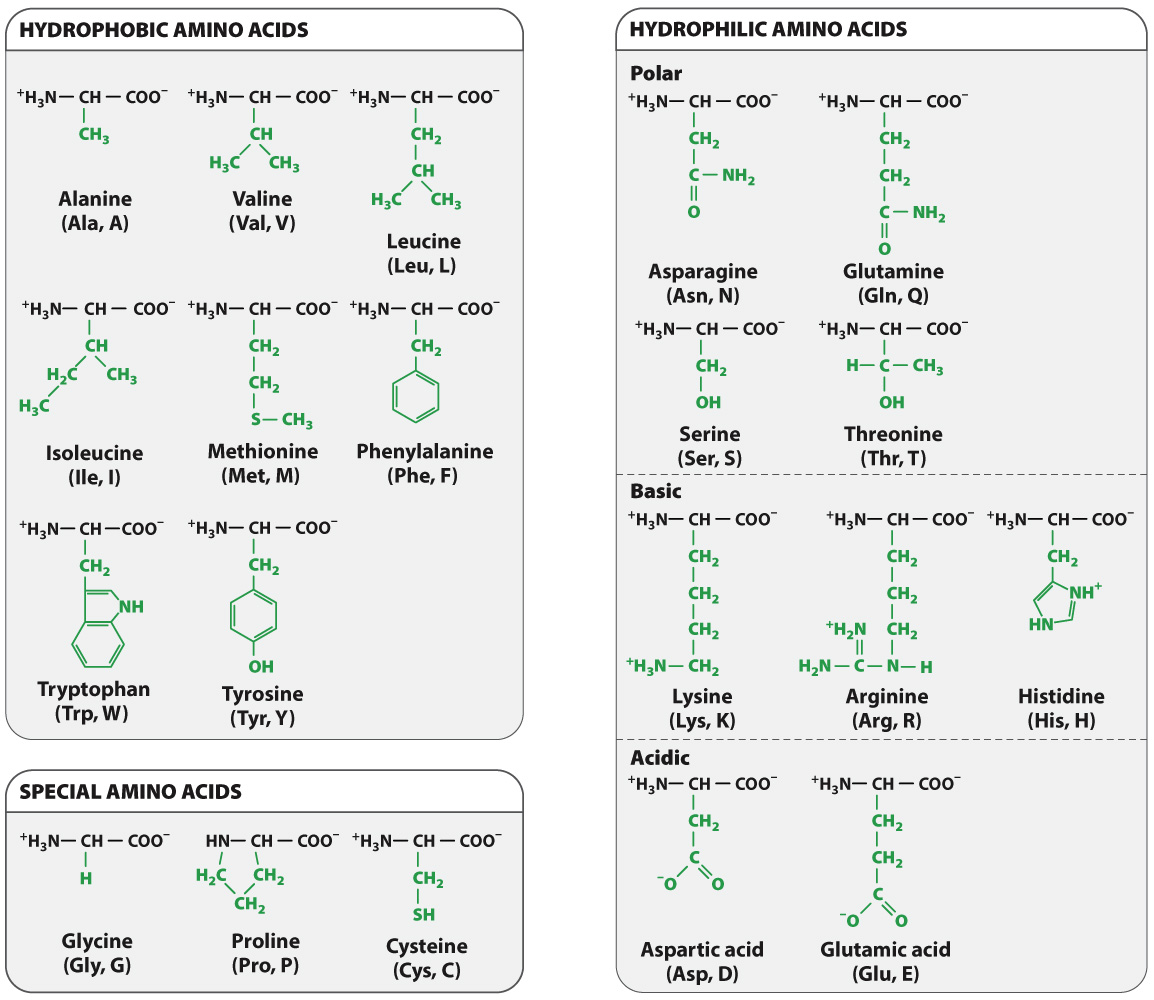
\includegraphics[scale=0.75]{background/aaformulas.jpg}\centering
    \caption[Amino acids formulas]{\label{fig:aaformulas}%
    \textbf{Amino acids formulas} --- from \citet{Morris2016-qv}}
\end{figure}

\section{Original material}\label{sec:kelvinsong}
\vspace{-5mm}
To create \Cref{fig:transcriptionTranslation},
I used original material
by Kelvinsong (\href{https://commons.wikimedia.org/wiki/User:Kelvinsong}{https://commons.wikimedia.org/wiki/User:Kelvinsong}):
\enquote{Simplified diagram of mRNA synthesis and processing. Enzymes not shown.}
(\href{https://commons.wikimedia.org/wiki/File:MRNA.svg}{https://commons.wikimedia.org/wiki/File:MRNA.svg})
and
\enquote{Protein synthesis} (\href{https://commons.wikimedia.org/wiki/File:Protein\_synthesis.svg}%
{https://commons.wikimedia.org/wiki/File:Protein\_synthesis.svg}).

\vspace{-3mm}
\section[EST-sequencing]{Expressed~Sequence~Tag~(EST)~sequencing}\label{sec:EST}
\vspace{-5mm}
\glspl{EST} are short nucleotide sequence generated
from randomly selected \gls{RNA} transcript~\mycite{Parkinson2009-pj}.
\mRNAs\ are reverse transcribed into double-stranded \glspl{cDNA}
(either from the 5' or 3' end of the transcript)~\mycite{Lowe2017-kj}.
These \glspl{cDNA} are cloned to create libraries~\mycite{Harbers2008-qh}
and then sequenced either by Sanger method~\mycite{Sanger1975-io} or
a more high-throughput one such as
the sequencing-by-synthesis (\Cref{subsub:sequencing}).
Although this technique is subject to sampling bias~\mycite{EST} and
often account for only 60\% of an organism expressed genes~\mycite{Bonaldo1996-lx},
it remains a relatively low cost alternative approach to study the transcriptome
(gene discovery).


\vspace{-3mm}
\section{Microarrays}\label{sec:microarray}
\vspace{-5mm}
Microarrays require prior knowledge
(\eg\ annotated genome or \glspl{EST} libraries)
of the organism of interest
as they exploit it to design \emph{probes} (short nucleotide oligomers)
that are arrayed on a solid support (\eg\ a glass or silicon thin film cell)%
~\mycite{Lowe2017-kj,Schena1995-tg,Bumgarner2013-ey}.
For transcriptome profiling,
the expressed \glspl{RNA} are first reverse transcribed into \glspl{cDNA}
(also referred as \emph{targets})
and then, after being fluorescently labelled, they are complimentary hybridised
to the microarray probes;
the relative abundance of the transcripts is assessed
by measuring the intensity of the fluorescence
after the excess of unhybridised \glspl{cDNA} is washed away~\mycite{Lowe2017-kj}.
This technology is extremely powerful and popular
as it allows global and parallel analyses of cellular activity.
Microarray technology also has many variations~\mycite{Hoheisel2006-lw}
in addition to its original \gls{cDNA} version
for transcriptional profiling~\mycite{Schena1995-tg}, \eg\
for genotyping~\mycite{Wang1998-rs,Gunderson2006-pp},
protein profiling~\mycite{Hall2007-gt,Sutandy2013-tj,Duarte2017-ao},
splice-variant analysis~\mycite{Cuperlovic-Culf2006-rg} or
transcription factor binding~\mycite{Bulyk2002-ii,Bulyk2007-jc} studies.

\clearpage
\section{FASTQ format}\label{sec:fastq-format}

\begin{figure}[!htbp]
\begin{minipage}[adjusting]{\textwidth}
{\small
{\color[rgb]{0.447059,0.678431,0.274510}\verb!@ERR030856.1!}
{\color[rgb]{0.500000,0.500000,0.500000}\verb!HWI-BRUNOP16X_0001:1:1:2669:1073#0!}%
{\color[rgb]{1.000000,0.000000,0.000000}\verb!/1!}\\
\verb!AAAGGATTATGCAGANGTAGGGCGTGTNNNNNNNNNNNNNGGCTGGGGNNNNNNNNNNNNNNNNNNATNNNCTGACCANCTGAAGTATGTCANGCTGCCT!\\
{\color[rgb]{0.698039,0.145098,0.450980}+}\\
{\color[rgb]{0.000000,0.000000,0.555711}\verb!HHHHHHHIHHFFFFF#>>@>GGGFG###########################################################################!}\\
{\color[rgb]{0.447059,0.678431,0.274510}\verb!@ERR030856.2!}
{\color[rgb]{0.500000,0.500000,0.500000}\verb!HWI-BRUNOP16X_0001:1:1:4476:1072#0!}%
{\color[rgb]{1.000000,0.000000,0.000000}\verb!/1!}\\
\verb!GATAGATTATCAGAANGACAGTTACTTNNNNNNNNNNNNNGGGCACTTNNNNNNNNNNNNNNNNNNATNNNTCATAAGNNCTGTTGCCAAATNAGTGATA!\\
{\color[rgb]{0.698039,0.145098,0.450980}+}\\
{\color[rgb]{0.000000,0.000000,0.555711}\verb!HHHHHHHHHHDDDDD#@@AAGGGGG###########################################################################!}
}
{\footnotesize
Legend:\\
\quad{\color[rgb]{0.447059,0.678431,0.274510}\textbullet\ Read identifier}\\
\quad{\color[rgb]{0.500000,0.500000,0.500000}\textbullet\ Optional information (here flow cell lane:tile number:x:y:z)}\\
\quad{\color[rgb]{1.000000,0.000000,0.000000}\textbullet\ First member of pair (here) or single-end}\\
\quad\textbullet\ Nucleotide sequence of the read\\
\quad{\color[rgb]{0.698039,0.145098,0.450980}\textbullet\ Separator (+ or any string of character)}\\
\quad{\color[rgb]{0.000000,0.000000,0.555711}\textbullet\ Phred score (here Phred 33)}
}
\end{minipage}
\caption{FASTQ format}\label{fig:fastqFormat}
\end{figure}

\FloatBarrier\

\section{Phred score}\label{sec:PhredScore}

\begin{table}[!htbp]
\centering
\caption{Phred quality score to accuracy significance}%
\label{PhredtoAccuracy}
\begin{tabular}{@{}lll@{}}
\toprule
\begin{tabular}[c]{@{}l@{}}Phred quality\\ score ($Q$)\end{tabular} & \begin{tabular}[c]{@{}l@{}}Probability of\\ incorrect\\ base call\end{tabular} & \begin{tabular}[c]{@{}l@{}}Base call\\ accuracy\end{tabular} \\ \midrule
10 & 1 in 10 & 90\% \\
20 & 1 in 100 & 99\% \\
30 & 1 in 1,000 & 99.9\% \\
40 & 1 in 10,000 & 99.99\% \\ \bottomrule
\end{tabular}
\end{table}

The \gls{Phred} quality score can be encoded in several standards as shown in \Cref{phredformat}.
%https://en.wikipedia.org/wiki/FASTQ_format#Encoding
\begin{figure}[htbp]
\begin{minipage}[adjusting]{\textwidth}
\begin{verbatim}
SSSSSSSSSSSSSSSSSSSSSSSSSSSSSSSSSSSSSSSSS.....................................................
..........................XXXXXXXXXXXXXXXXXXXXXXXXXXXXXXXXXXXXXXXXXXXXXX......................
...............................IIIIIIIIIIIIIIIIIIIIIIIIIIIIIIIIIIIIIIIII......................
.................................JJJJJJJJJJJJJJJJJJJJJJJJJJJJJJJJJJJJJJJ......................
LLLLLLLLLLLLLLLLLLLLLLLLLLLLLLLLLLLLLLLLLL....................................................
!"#\$\%&'()*+,-./0123456789:;<=>?@ABCDEFGHIJKLMNOPQRSTUVWXYZ[\]^_`abcdefghijklmnopqrstuvwxyz{|}~
 |                         |    |        |                              |                     |
33                        59   64       73                            104                   126
 0........................26...31.......40
                          -5....0........9.............................40
                                0........9.............................40
                                   3.....9.............................40
 0........................26...31........41

S - Sanger        Phred+33, raw reads scores between  0 and 40
X - Solexa        Phred+64, raw reads scores between -5 and 40
I - Illumina 1.3+ Phred+64, raw reads scores between  0 and 40
J - Illumina 1.5+ Phred+64, raw reads scores between  3 and 40
        with 0=unused, 1=unused, 2=Read segment Quality Control Indicator
L - Illumina 1.8+ Phred+33, raw reads scores between  0 and 41
\end{verbatim}
\end{minipage}
\caption{The available Phred score quality score encoding formats}\label{phredformat}
\end{figure}

\begin{figure}[!htbp]
    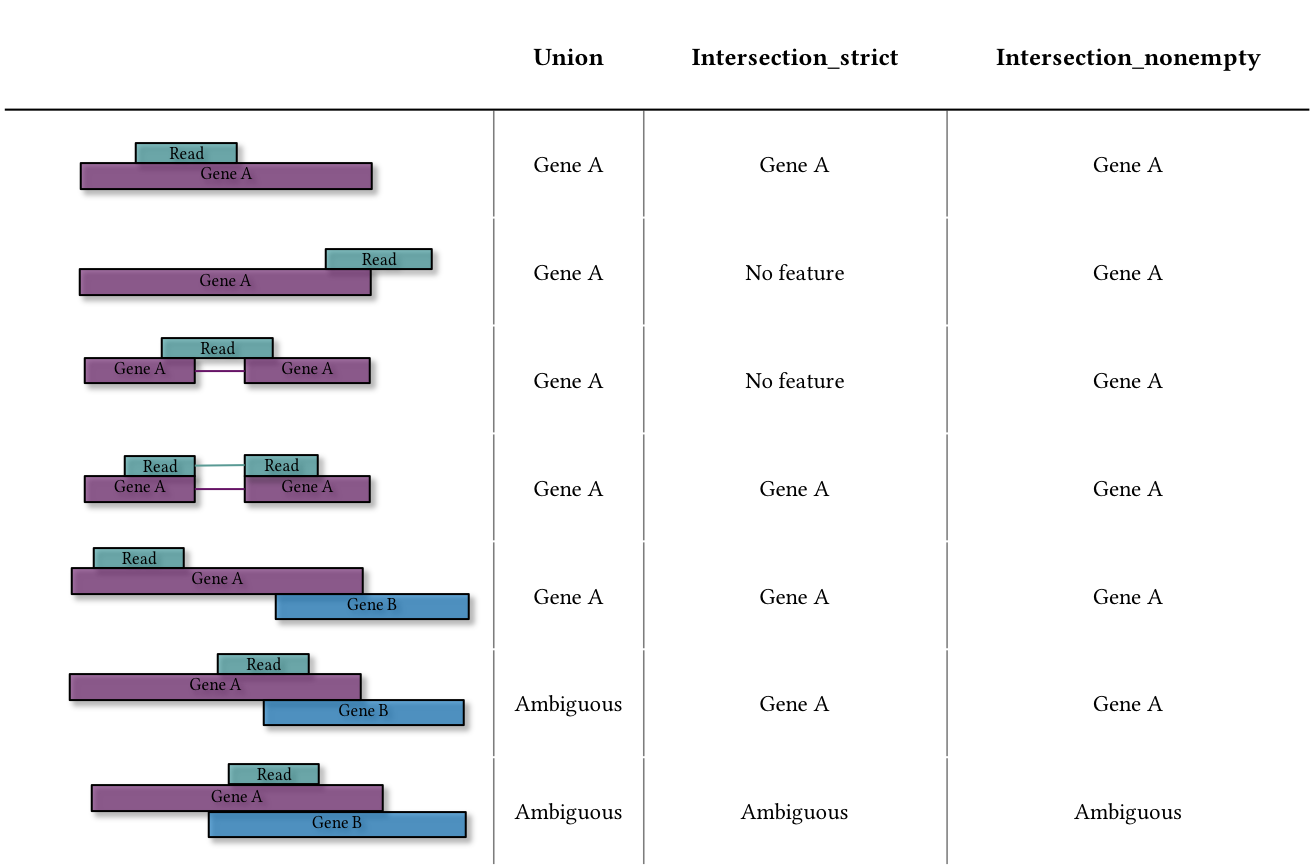
\includegraphics[scale=0.60]{background/interestHtseq}\centering
    \caption[Overlap resolution effects for each \htseq\
    mode]{\label{fig:htseqMode}\textbf{Overlap resolution effects for each \htseq\
    mode.} Each mode resolves a number of overlap situations differently. The
    mode used in this thesis is the \texttt{intersection non-empty} mode. This
    specific mode resolves more situations than the two others. Hence, the loss
    of ambiguous reads is reduced in this mode. [Adaptated from HTseq
    documentation: \footnotesize{\href{http://www-huber.embl.de/HTSeq/doc/count.html}%
    {http://www-huber.embl.de/HTSeq/doc/count.html}}]}
\end{figure}


\begin{table}[]
\centering
\caption{\gls{FPKM} are unsuitable for differential expression analysis}%
\label{tab:noFPKM4DEA}
\begin{tabular}{@{}lcccc@{}}
\toprule
\multicolumn{1}{l|}{} & \multicolumn{2}{c|}{Sample 1} & \multicolumn{2}{c}{Sample 2} \\ \midrule
\multicolumn{1}{l|}{} & \multicolumn{1}{c|}{raw counts} & \multicolumn{1}{c|}{normalised counts} & \multicolumn{1}{c|}{raw counts} & normalised counts \\ \midrule
\multicolumn{1}{l|}{$Gene_{1}$} & \multicolumn{1}{c|}{100} & \multicolumn{1}{c|}{0.010} & \multicolumn{1}{c|}{80} & 0.008 \\
\multicolumn{1}{l|}{$Gene_{2}$} & \multicolumn{1}{c|}{100} & \multicolumn{1}{c|}{0.010} & \multicolumn{1}{c|}{80} & 0.008 \\
\multicolumn{1}{c}{\ldots} & \ldots & \ldots & \ldots & \ldots \\
\multicolumn{1}{l|}{$Gene_{i}$} & \multicolumn{1}{c|}{100} & \multicolumn{1}{c|}{0.010} & \multicolumn{1}{c|}{80} & 0.008 \\
\multicolumn{1}{l|}{$Gene_{i+1}$} & \multicolumn{1}{c|}{0} & \multicolumn{1}{c|}{0} & \multicolumn{1}{c|}{2000} & 0.2 \\ \midrule
\begin{tabular}[c]{@{}l@{}}Total number\\ of fragments ($F$)\end{tabular} & 10,000 & 1 & 10,000 & 1 \\ \bottomrule
\end{tabular}
\end{table}

\FloatBarrier\


\section{Mass analysers}\label{sec:appMassAnalysers}

See~\citet{Haag2016} for more details on other types of analysers.

\minisec{Quadrupole analyser}
It is one of the most popular analysers as they are cheap compared to the
others. They are also compact, durable and reliable. The quadrupole analyser can
filter the ions based on their difference of $m/z$. They are adequately
named quadrupole as they comprise four cylindrical or hyperbolic rods in
parallel to each other. Opposite rods are connected together electrically and
\gls{RF} potential is applied. A \gls{DC} potential is superimposed on the
\gls{RF} one. These combinations of \gls{RF} and \gls{DC} potentials constrain the
ions to oscillate between the rods as they pass through them. Hence, by tuning
the \gls{RF} and \gls{DC}, it is easy to select for which range of $m/z$ ions
will have a stable trajectory and thus the only one detected. Indeed, the
ions with unstable trajectory will collide with the rods and be \enquote{filtered}
out. If used in \enquote{\gls{RF}-only} mode (\gls{DC} reduced to a minimum),
the quadrupole may have other applications. For example, it can guide specific
$m/z$ ions to other areas (while the bulk of ions will remain trapped).
It may also be used as collision cells for \gls{CID}: by introducing an inert
gas and tuning with the \gls{RF}-energy, the amount of fragmentation undergone
by the targeted ions can be precisely controlled. \mycite{Haag2016}\\
The quadrupole analyser is also qualified as the \emph{mass filter}.

\minisec{\Acrfull{LTQ}}
\gls{LTQ} is a particular kind of \acrfull{LIT} which is in principle a sort of
a quadrupole mass analyser~\mycite{Zhang2014}. A \gls{LTQ} uses a set of
quadrupole rods and a two-dimensional \gls{RF} field confines the ions radially.
In addition, a static electrical potential is applied to end electrodes which
forbid the ions to escape axially. However, the quadrupole is commonly segmented
into three parts which ensure a perfect homogeneity of the electric field of the
trap area and thus avoiding ion loss when the trapping is done.
While they may be used as an ion trap, they
may be also used as a simple mass filter. \gls{RF} voltage is tuned to produce
multi-frequency resonance ejection waveforms are applied as to
eliminate all the undesirable ions in the trap before the fragmentation and mass
analysis of the remaining ones. Frequently, these \glspl{LTQ} are used as a
front-end to other mass analysers as they have high injection efficiencies and
high ion storage capacities. They may be equipped then with two biased radial
ejection slits and then be used with two detectors hence the signal-to-noise
ratio may be doubled.

Compared with other traps, linear ion traps provide an enhanced dynamic range
with a reduced low mass cut-off as the ion cloud is
spatially distributed on a linear axis and not a 3D centre which improves the
sensitivity. And then, for example, the ions may then be accumulated before
being released into another mass analyser~\mycite{Madalinski2008}.

\minisec{\orbi}
It is a very recent analyser and it relies on \gls{FT}. Recently,
there is increasing use of \glspl{FTMS} for proteomic studies. Indeed, these
\glspl{FTMS} are more precise than previous analysers and allow the detection of
a greater range of ions in very short lapses of time~\mycite{Scigelova2011}.
In this kind of analyser, ions are trapped and both orbit around and oscillate
in an electrostatic field between an inner and outer part of a central electrode
shaped as a spindle.
The ions can only move following the spindle long axis~\mycite{Makarov2000}.
While moving around the spindle the ions create a current.
The outer part of the spindle records images of this current.
Fourier transformation of these images allows obtaining very highly accurate
and sensitive mass spectra for a greater dynamic range than most of the
other analysers.~\mycite{Hu2005}

\minisec{\gls{LTQ}-\orbi}
It is a hybrid (tandem) mass spectrometer that uses \gls{ESI} for the ionisation
step and has an \gls{LTQ} as a first analyser (MS$^1$)
and an \orbi\ as a second one (MS$^2$).
This \gls{MS/MS} enables multiple levels of
fragmentation for the elucidation of a wide range of peptides and can be coupled
with an \gls{ESI} which is a continuous source of ionisation. This instrument
allows analysing proteomic samples optimally both in terms of starting material,
time~\mycite{Scigelova2011} and provides \enquote{ultrahigh} mass resolution,
high mass accuracy
and enhanced dynamic range with respect to mass accuracy~\mycite{Madalinski2008}.

\section{Isotopes of common elements and their natural
frequency}\label{app:isotopes}
\Cref{tab:isotope} lists the mass~\mycite{Audi1993-qn,Audi1995-uk}
and the percent natural abundance~\mycite{Rosman1998-xu}
for stable nuclides (\ie\ atom distinctly characterised by its number of protons (Z)
and number of neutrons (N)) that may be found in \glspl{DNA}, \glspl{RNA} and proteins.

\begin{table}[!htbp]
\centering
\caption[Most common elements and their stable isotopes]%
{\textbf{Most common constitutive elements and their stable isotopes\\ found in DNAs,
RNAs and proteins.} Asterisks (*) mark abundances that are not available.
Adapted from~\mycite{Audi1993-qn,Audi1995-uk,Rosman1998-xu}
}%
\label{tab:isotope}
\begin{tabular}{@{}clccr@{}}
\toprule
\begin{tabular}[c]{@{}c@{}}%
    z \\ (Atomic number)\end{tabular} &
    \multicolumn{1}{c}{Name} & Isotope &
    \begin{tabular}[c]{@{}c@{}}Mass atomic\\ (u)\end{tabular} &
        \multicolumn{1}{c}{\begin{tabular}[c]{@{}c@{}}Natural frequency\\ (\%)\end{tabular}} \\
\midrule
1  & Hydrogen & \isotope[1]{H} & 1.007825 & 99.9885 \\
   & Deuterium & \isotope[2]{H} & 2.014102 & 0.0115 \\
   & Tritium & \isotope[3]{H} & 3.016049 & * \\
6  & Carbon & \isotope[12]{C} & 12.000000 & 98.93 \\
   &  & \isotope[13]{C} & 13.003355 & 1.07 \\
   &  & \isotope[14]{C} & 14.003242 & * \\
7  & Nitrogen & \isotope[14]{N} & 14.003074 & 99.632 \\
   &  & \isotope[15]{N} & 15.000109 & 0.368 \\
8  & Oxygen & \isotope[16]{0} & 15.994915 & 99.757 \\
   &  & \isotope[17]{0} & 16.999132 & 0.038 \\
   &  & \isotope[18]{0} & 17.999160 & 0.205 \\
15 & Phosphorus & \isotope[31]{P} & 30.973762 & 100 \\
16 & Sulphur & \isotope[32]{S} & 31.972071 & 94.93 \\
   &  & \isotope[33]{S} & 32.971458 & 0.76 \\
   &  & \isotope[34]{S} & 33.967867 & 4.29 \\
   &  & \isotope[35]{S} & 35.967081 & 0.02 \\
53 & Iodine & \isotope[127]{I} & 126.904468 & 100 \\
\bottomrule
\end{tabular}
\end{table}

\section{Hypothesis testing}\label{pq-values}

\subsection{$\mathcal{H}_0$}\label{H0}
In statistical testing,
the null hypothesis $\mathcal{H}_0$ is an answer
to the intrinsic nature of statistical calculation:
the smaller a given interval is,
the lower the probability of a simple random draw in that interval.
The null hypothesis can be of different natures.
It is generally formulated as an absence of difference
between two objects to be compared,
or as an absence of relationship between two variables of a same population;
its purpose is to be rejected.
It is always opposed to another \emph{alternative} hypothesis ($\mathcal{H}_1$),
which is accepted when $\mathcal{H}_0$ is rejected.

To test an hypothesis,
one needs to construct a statistical model that can represent an ideal form
of the data if it were to be generated by random processes alone.
This model is also referred as the \emph{distribution under the null hypothesis}.
Then, the likelihood of the collected (observed) data is computed.
Finally, it is compared to the (random) probability determined by the model
to either accept $\mathcal{H}_0$ or reject it
if the observed data is very unlikely under the null hypothesis.
Usually a test statistic
(\ie\ quantity derived from the sample used for the hypothesis testing)
that measures the apparent departure from the null hypothesis is compared
to a value defined such as the probability of a \enquote{more extreme value}
is even smaller under the null hypothesis.
Prior to the analysis, an arbitrary level of significance (or $\alpha$) is
set either to 0.1, 0.05, 0.01, 0.005 or 0.001,
\ie\ 10\%, 5\%, 1\%, 0.5\% or 0.1\% risk to reject $\mathcal{H}_0$ by mistake.

Depending on whether the observed data is tested, case (1): in both direction,
\ie\ the data is either \emph{greater or equal} to the critical value ($x$) or
\emph{lesser or equal} to the additive inverse of the critical value ($-x$),
or, case (2) in one direction only,
\ie, (for example) the data is (only) \emph{greater or equal} to the critical value
(or the data is (only) \emph{lesser or equal} to the critical value),
the statistical test is two-tailed (case 1) or one-tailed.

\subsection{p-value}\label{p-value}
In statistical hypothesis testing,
the p-value quantifies the statistical significance of results,
under the null hypothesis $\mathcal{H}_0$ (see \Cref{H0}).
It allows rejecting (or not) $\mathcal{H}_0$.
The p-value is the probability for a given statistical model of obtaining
an equal value or an even more extreme value than what has been observed
when $\mathcal{H}_0$ is true.
Depending on the situation,
the more extreme value can mean:
\begin{eqlist}
        \item[One-tail event]
            \begin{eqlist}
            \item[Left tail event]  $\text{Pr}(X \leq x \mid \mathcal{H}_0)$
            \item[Right tail event] $\text{Pr}(X \geq x \mid \mathcal{H}_0)$
            \end{eqlist}
        \item[Two-tail event] $2\text{min}(\text{Pr}(X \leq x \mid \mathcal{H}_0),%
            \text{Pr}(X \geq x \mid \mathcal{H}_0))$
\end{eqlist}
The smaller is a p-value,
the higher the significance, \ie\
the stronger the evidence that $\mathcal{H}_0$ has to be rejected.
$\mathcal{H}_0$ is rejected if the adequate probability is less than or equal to
an arbitrary pre-defined (\ie\ prior to the analysis) threshold value $\alpha$.

Under $\mathcal{H}_0$,
the assumption is that the p-values are uniformly distributed.\mybr\

\subsection{q-value}\label{q-value}\label{multitesting}
A q-value is an adjusted p-value
(which the calculation may or may not be based on the p-value).
In the context of multi-testing,
\ie\ when multiple simultaneous statistical tests occur,
the likelihood of rejecting $\mathcal{H}_0$ due to a random sampling increases.
To avoid accepting the alternative hypothesis by mistake,
the whole p-values collection is tested and adjusted for \glsentrydesc{FDR}.
A q-value of 5\% means that 5\% of all the significant results
are actually false positives.

\section{One example of normalisation factor for proteomic data}

\begin{minipage}{\textwidth}

\begin{equation}\label{eq:NSAF}
       \tag{\gls{NSAF}}
       \text{NSAF} = \frac{\frac{\text{SpC}_p}{\text{Length}_p}}{%
       \sum_{i=1}^N \frac{\text{SpC}_i}{\text{Length}_i}
       }
\end{equation}

where:
{\small
\begin{itemize}
        \item $\text{SpC}$ is the number of acquired spectra for a protein (Spectral count)
        \item $\text{Length}$ is the length of a protein (can be its molecular weight)
        \item $p$ is the index of the currently considered protein
%        \item $\sum_{i=1}^N \frac{\text{SpC}_i}{\text{Length}_i}$ is the sum of all
%            $\frac{\text{SpC}}{\text{Length}}$ of all the proteins of the sample.
        \item N is the total number of identified proteins in the sample
\end{itemize}
}

\end{minipage}
